\documentclass[paperwidth=40in,paperheight=32in,margin=1in,fontscale=0.33]{baposter}
\usepackage{amsmath}
\usepackage{amssymb}
\usepackage{enumitem}
\usepackage{subcaption}
\usepackage{float}
\usepackage{graphicx}
\usepackage[numbers]{natbib}
\usepackage{xcolor}
\usepackage{tikz}
\usepackage{pgfplots}
\usepackage[font=normalsize,labelfont=bf]{caption}


% \frenchspacing

\definecolor{box_color}{RGB}{126, 223, 231}
\definecolor{header_left}{RGB}{67, 148, 225}
\definecolor{header_right}{RGB}{77, 132, 199}
\definecolor{bg}{RGB}{215, 134, 57}


\renewcommand{\P}{\mathbb{P}}
\newcommand{\V}{\mathcal{V}}
\newcommand{\R}{\mathbb{R}}
\newcommand{\Z}{\mathbb{Z}}


\DeclareMathOperator*{\argmin}{arg\,min}
\DeclareMathOperator*{\argmax}{arg\,max}

\DeclareMathOperator{\tr}{tr}



\setlist{nolistsep} % more compact spacing between environments
\setlist[itemize]{leftmargin=*} % nice margins for itemize ...

\setlength{\fboxsep}{1mm}

\begin{document}
\begin{poster}{
    headerColorOne=header_left, %
    headerColorTwo=header_right, %
    boxColorOne=box_color, %
    textborder=none, %
    headerborder=none, %
    background=plain, %
    bgColorOne=bg!10, %
    %% headers
    headerfont=\Large\sf\bf, %
    headerheight=0.11\textheight, %
    headershape=rounded, %
    %% other
    columns=3,
    grid=true}{}{
	\Huge arXiv vs. snarXiv}{
	\Large Tyler Blanton and Sam Kowash\\University of Washington, Department of Physics}{
\includegraphics[height=.75in]{figures/uw_block_purple.eps}}

\headerbox{Background}{name=background,column=0,row=0,span=2}{
	The arXiv is a popular e-print repository for publications in physics, astronomy, and other quantitative sciences. It hosts nearly 1.5 million papers, of which $\sim$120,000 are in theoretical high-energy physics (\texttt{hep-th}). Physicist David {Simmons-Duffin} developed a program known as the snarXiv, which procedurally generates abstracts in the style of \texttt{hep-th} from a context-free grammar.

	Humans (even physicists) have surprising difficulty determining whether a given abstract is from the arXiv or the snarXiv. Over 750,000 guesses collected through an online sorting game, players succeeded at picking the genuine paper from a pair only 59\% of the time. Try it for yourself below!\vspace{.25\baselineskip}


	\fcolorbox{black}{white}{
	\begin{minipage}[t]{.47\textwidth}
		{\small\bf Abstract A}

		\footnotesize
		In the 20th century, a fair amount of work was done demystifying QED in the presence of a stack of canonical co-isotropic branes. In this paper, we make contact with analyzing heterotic strings, consequently reconstructing perturbation theory on $\mathbb{C}^n$, and classify anomalous dimensions in loop models with sleptons. Our computation of the solution of magnetic dualities in models of hadrons provides a certain notion of perturbation theory (taking into account cosmic rays at $\Lambda_\mathrm{QCD}$). Our results prove that decay constants turn out to be equivalent to an instanton at the Planck scale. Finally, we establish that sleptons can be brought to bear in reformulating heavy ions.
		\vspace{.2\baselineskip}
	\end{minipage}}
	%
	\fcolorbox{black}{white}{
	\begin{minipage}[t]{.47\textwidth}
		{\small\bf Abstract B}

		\footnotesize
		We study the effective action of the heterotic string compactified on particular half-flat manifolds which arise in the context of mirror symmetry with NS-NS flux. We explicitly derive the superpotential and K{\"a}hler potential at lowest order in $\alpha'$ by a reduction of the bosonic action. The superpotential contains new terms depending on the K{\"a}hler moduli which originate from the intrinsic geometrical flux of the half-flat manifolds. A generalized Gukov formula, valid for all manifolds with SU(3) structure, is derived from the gravitino mass term. For the half-flat manifolds it leads to a superpotential in agreement with our explicit bosonic calculation. We also discuss the inclusion of gauge fields.
	\end{minipage}
	}

	\vspace{0.25\baselineskip}
	We explored computational approaches to this classification problem to investigate whether its difficulty stems from snarXiv's genius, or humans' bewilderment in the face of unfamiliar jargon.
}



\headerbox{$n$-gram model}{name=ngram,column=0,row=0.38,span=1}{%
	One approach to text classification is to develop a \emph{language model}. Given a class $Y \in \{-1,1\}$ (with the negative sign referring to arXiv and the positive to snarXiv) and a document $X$ consisting of words $\{w_i\}_{i=1}^N$, we want to characterize the probability
	\vspace{-.5em}
	\begin{align*}
		\P(X | Y) &= \prod_{i=1}^N \P(w_i|w_1^{i-1}, Y),
	\end{align*}
	%
	where $w_1^{i-1}$ is the sequence of the first $i-1$ words. The sample space dwarfs the available data and this can never be satisfactorily trained. Instead we assume that a word's probability depends only on the preceding $n-1$ words, reducing the training task to estimating the probabilities of so-called $n$-grams from their frequencies in the training corpora.
	\vspace{-.5em}
	\begin{align*}
		\hat{\P}(X|Y) \equiv \prod_{i=1}^N \hat{\P}(w_i | w_{i-n+1}^{i-1}, Y) \equiv \frac{C_Y(w_{i-n+1}^i)+1}{C_Y(w_{i-n+1}^{i-1}) + V},
	\end{align*}
	%
	where $C_Y(w_{i-n+1}^i)$ is the number of times that $n$-gram occurs in the corpus for class $Y$ and $V$ is the size of our vocabulary. In our experiments we studied 1-grams (known as the bag-of-words model) and 2-grams.
	}


\headerbox{Naive Bayes}{name=nb,column=0,row=.84}{
	The simplest classifier based on $n$-gram frequencies sorts a document into whichever class has a higher posterior probability based on our estimate:
	\vspace{-.5em}
	\begin{align*}
		\hat{Y} &= \argmax_{Y\in\{-1,1\}} \P(Y) \hat{\P}(X|Y),
	\end{align*}
	%
	where $\P(Y)$ is the fraction of training abstracts in class $Y$.
}	

\headerbox{Likelihood-ratio test}{name=lr,column=1,row=.38}{
	The LR test improves upon naive Bayes by giving us a hyperparameter $\eta$ to adjust the sensitivity of the test. Given the ratio $\Lambda(X) \equiv \hat{P}(X|Y=1)/\hat{P}(X|Y=-1)$, the classifier $\delta^\ast_{LR}$ chooses class 1 (snarXiv) with probabilities
	%
	\begin{align*}
		\P(\delta^\ast_{LR}(X) = 1) &= \begin{cases}
									   	1, & \Lambda(X) > \eta\\
									   	1/2, &\Lambda(X) = \eta\\
									   	0, &\Lambda(X) < \eta\\
									   \end{cases}.
	\end{align*}
	%
	This reduces to the previous case when $\eta$ is the ratio of arXiv abstracts to snarXiv in the training set.
}


\headerbox{tf--idf}{name=tfidf, column=1, row=.64}{
	Another approach is to map documents into a continuous vector space and apply a method such as logistic regression to classify. We used a tf--idf method, where each document gets a vector $d$ with an entry $d_i$ for each word in the vocabulary, weighted by
	%
	\begin{align*}
		d_i &= \mathrm{tf}_{i,d} \cdot \mathrm{idf}_i
	\end{align*}
}


\headerbox{References}{name=refs,column=2,row=0.9,span=1}{}





% \headerbox{tf--idf}{name=tfidf,column=1,row=0.0}{%
% }




\setlength{\fboxsep}{0mm}
\headerbox{Results}{name=results,column=2,row=0, span=1}{
\textbf{\underline{Naive bayes classifier}}: $\text{TCA} \approx 77\%$ ($\text{TPR} = 100\%$, $\text{FDR} \approx 32\%$)
\\
\textbf{\underline{Likelihood-ratio test}:} $\text{TCA} \approx 99.98\%$ for $\eta_\text{PP}=1.4$
	\vspace{-1em}
	\begin{figure}[H]
		\centering
		\fbox{\begin{subfigure}[t]{.49\textwidth}
			\centering
			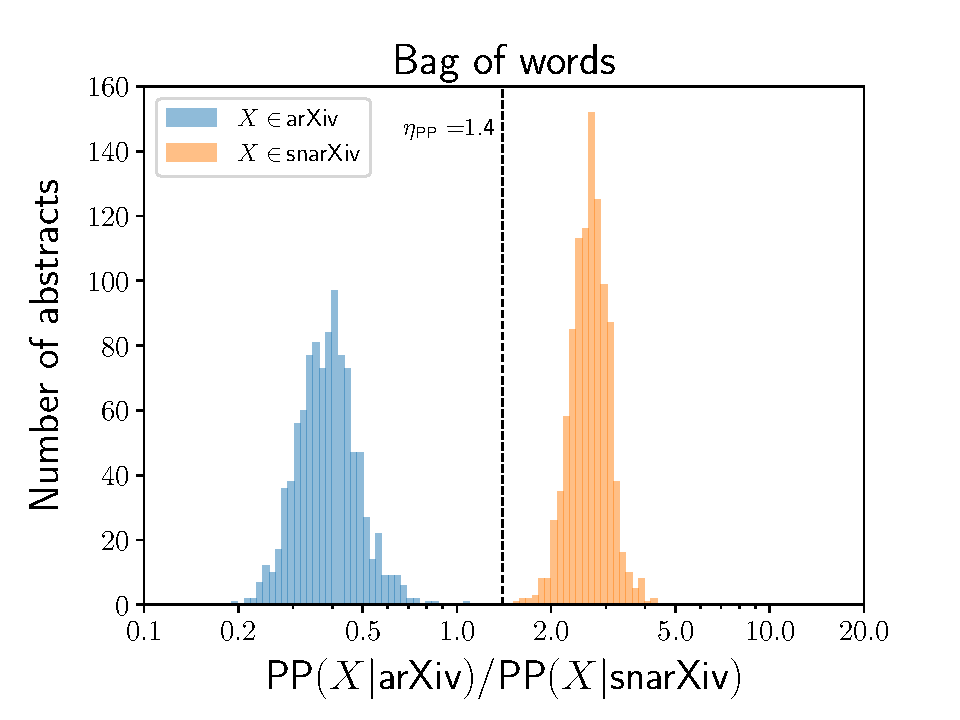
\includegraphics[width=\textwidth]{figures/BoW_histogram.pdf}
		\end{subfigure}}
		%
		\fbox{\begin{subfigure}[t]{.49\textwidth}
			\centering
			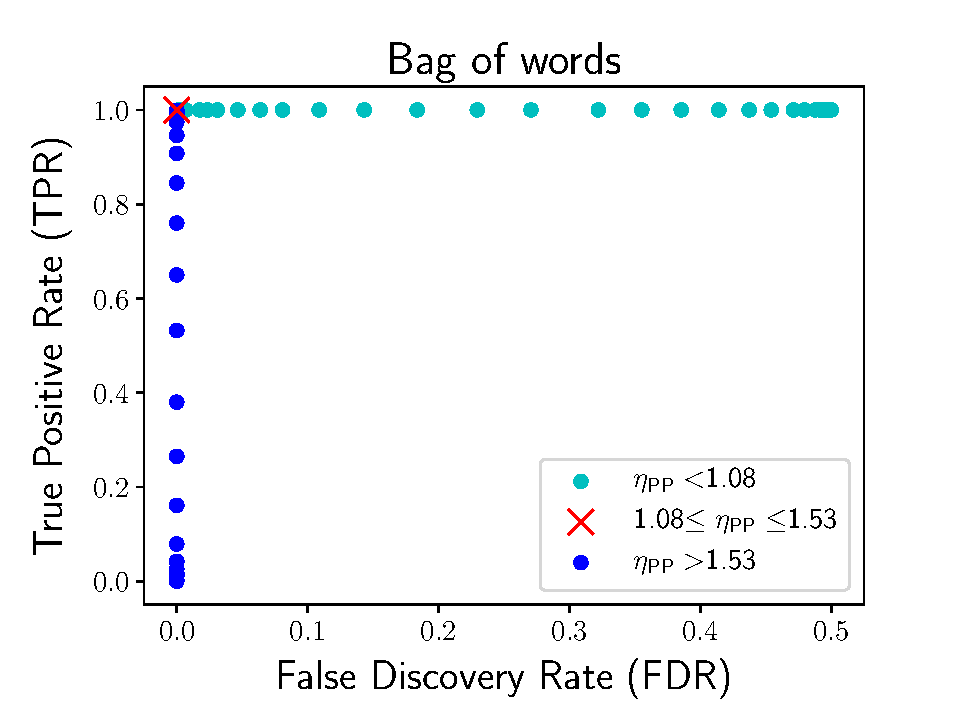
\includegraphics[width=\textwidth]{figures/BoW_TPR_FDR.pdf}
		\end{subfigure}}

		\fbox{\begin{subfigure}[t]{.49\textwidth}
			\centering
			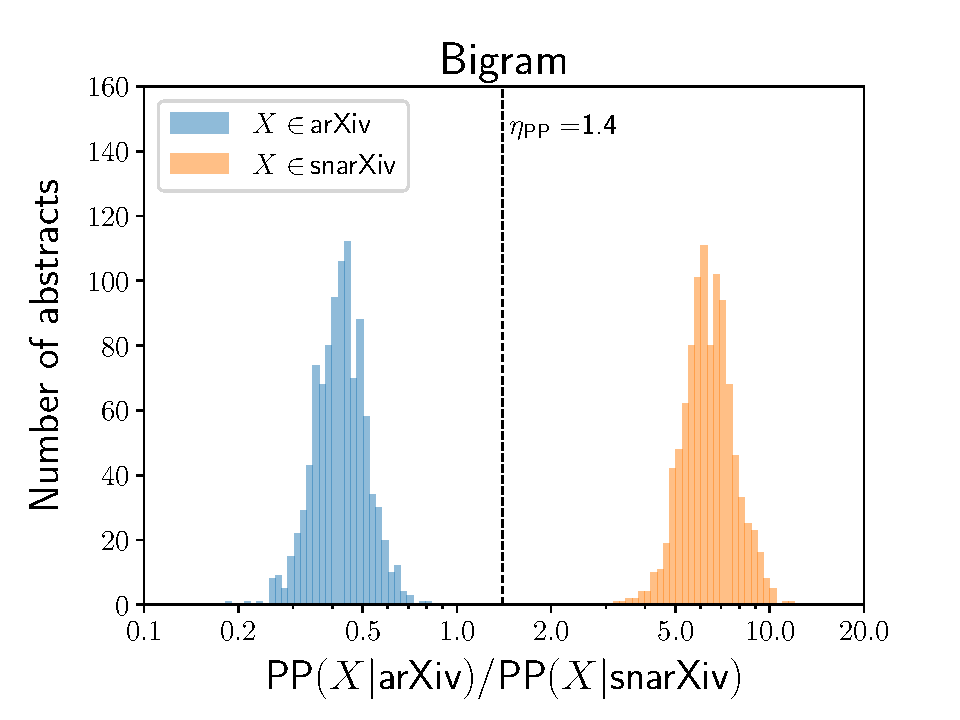
\includegraphics[width=\textwidth]{figures/bi_histogram.pdf}
		\end{subfigure}}
		%
		\fbox{\begin{subfigure}[t]{.49\textwidth}
			\centering
			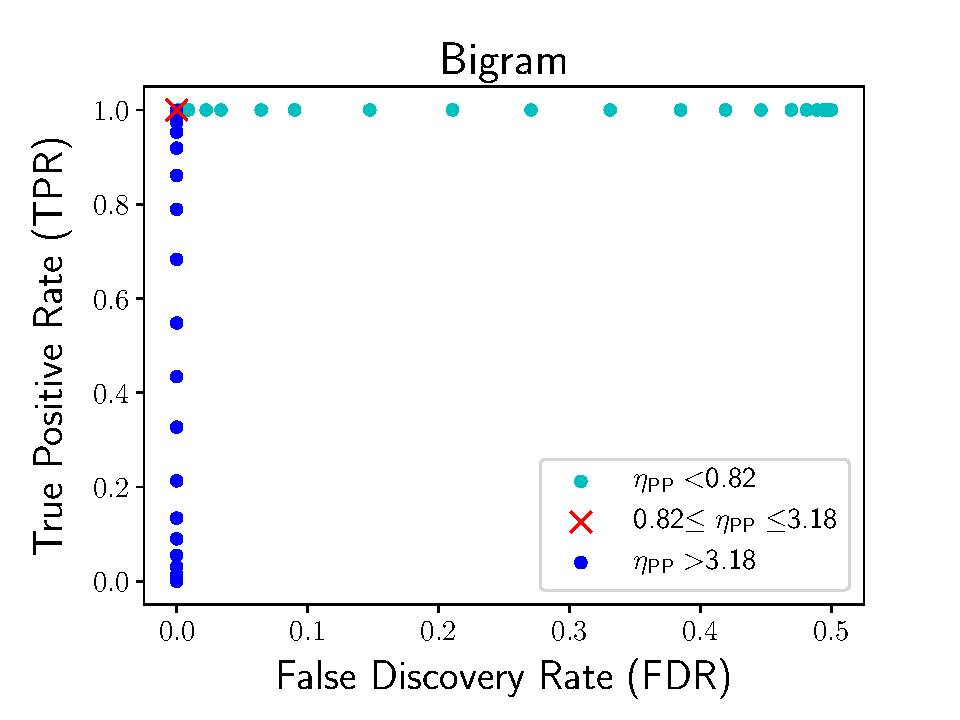
\includegraphics[width=\textwidth]{figures/bi_TPR_FDR.pdf}
		\end{subfigure}}
	\end{figure}
%
\textbf{\underline{tf--idf + logistic regression}:} $\text{TCA} \approx 99.96\%$ for $\lambda=2.5\times10^{-8}$
\\

For each model, we trained on 1,000 arXiv + 1,000 snarXiv abstracts and tested on 4,000 arXiv + 4,000 snarXiv abstracts, using a vocabulary of 15,315 unique words that appeared at least twice in a separate training corpus of 12,000 arXiv + 12,000 snarXiv abstracts.

The naive Bayes classifier (using bag-of-words) is by far the worst performer, having a total classification accuracy (TCA) of just 77\% due to its high propensity for false positives.
The likelihood-ratio test (for both bag-of-words and bigrams) and logistic regression (on tf--idf) are both able to almost completely resolve this issue, each sporting a TCA greater than $99.95\%$.

Comparing the bag-of-words and bigram models in the likelihood-ratio test, we find that both of the resulting classifiers are able to achieve a TCA of at least $99.98\%$ for appropriate choices of $\eta_\text{PP}$, the range of $\eta_\text{PP}$ which achieve these accuracies is significantly wider in the bigram model; in other words, adding context to words makes the contrast between arXiv and snarXiv abstracts much more pronounced.
}
\setlength{\fboxsep}{1mm}



% \headerbox{Conclusions}{name=conclusions, column=1, row=.75}{
	
% }





% \headerbox{References}{name=refs,column=2,row=.8}{
% 	\begingroup
% 	\renewcommand{\section}[2]{}
% 	\bibliographystyle{plainnat}
% 	\bibliography{lag_paper_new}
% 	\endgroup
% }

\end{poster}
\end{document}